\subsubsection{Software Integration Sequence}
In order to show the sequence of the integration, we distinguish into the two subsystem server and client.

\newpage
\paragraph{Server}\mbox{}
\newline 
The next figure will show the sequence of the integration of the components of the server.
\newline

\begin{figure}[H]
    \centering
    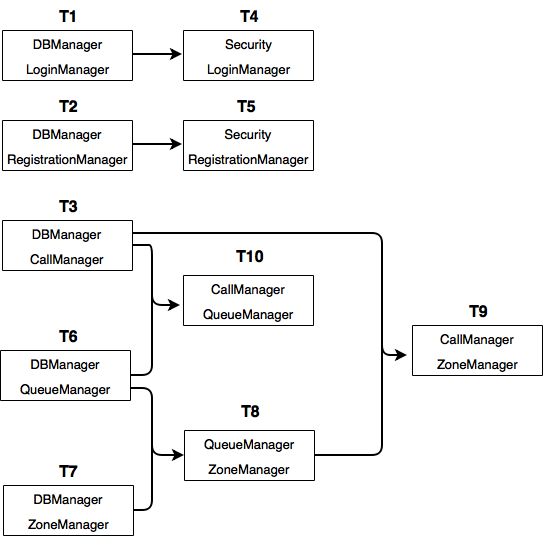
\includegraphics[width=13cm]{./Images/System-2.png}
    \caption{Sequence of integration in the server}
    \label{fig: Sequence of integration in the server}
\end{figure}
\newpage

\paragraph{Client}\mbox{}
\newline
The next figure will show the sequence of the integration of the components of the client.
\newline
In particular, we want to underline that we decided to give priority to tests that concern taxi drivers; indeed, those tests will be performed before the ones regarding passengers. This choice is due to the fact that in our project the central role is played by taxi rather than passengers. 
\newline
\begin{figure}[H]
    \centering
    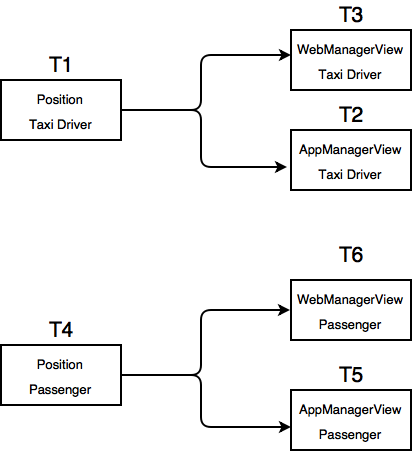
\includegraphics[width=11cm]{./Images/Client.png}
    \caption{Sequence of integration in the client}
    \label{fig: Sequence of integration in the client}
\end{figure}

\newpage

\subsubsection{Subsystem Integration Sequence}
The next figure will show the sequence of the integration of the main subsystems.
\newline
The integration of subsystems will start from the database and the server; then, we will integrate the server and the client. This choice seems reasonable since the database and the server are the most important parts of the hole system: the server manages the business logic, while the database manages the data. So, we decided to give highest priority to this two subsystems rather than the client.
\newline
\begin{figure}[H]
    \centering
    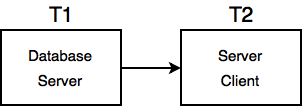
\includegraphics[width=9cm]{./Images/Subsystem.png}
    \caption{Sequence of integration of the subsystems}
    \label{fig: Sequence of integration of the subsystems}
\end{figure}